\documentclass{beamer}
\usepackage[utf8]{inputenc}

\usepackage{amsmath}
\usepackage{graphicx}
\usepackage{url}
\usepackage{fancyvrb}
\usepackage{xcolor}

\usetheme{Antibes}
\usecolortheme{whale}
\usepackage{lmodern}

\usepackage{listings}
\usepackage{color}

\definecolor{codegreen}{rgb}{0,0.6,0}
\definecolor{codegray}{rgb}{0.5,0.5,0.5}
\definecolor{codepurple}{rgb}{0.58,0,0.82}
\definecolor{backcolour}{rgb}{0.95,0.95,0.92}

\mode<presentation>

\definecolor{orange}{HTML}{BC2E07}

\usepackage{hyperref}
\hypersetup{
    colorlinks,
    linkcolor=orange,
    urlcolor=blue
}

\lstdefinestyle{mystyle}{
    language=C++,
    basicstyle=\ttfamily\footnotesize,
    backgroundcolor=\color{backcolour},
    commentstyle=\color{codegreen},
    keywordstyle=\color{magenta},
    numberstyle=\tiny\color{codegray},
    stringstyle=\color{codepurple},
    breakatwhitespace=false,
    breaklines=true,
    captionpos=b,
    keepspaces=true,
    numbers=left,
    numbersep=5pt,
    showspaces=false,
    showstringspaces=false,
    showtabs=false,
    tabsize=2
}

\title{Lab \# 3: I/O Programming}
\subtitle{EC-102 -- Computer Systems and Programming}

\author{Usama Wajhi}
\institute{School of Mechanical and Manufacturing Engineering (SMME), \\ National University of Sciences and Technology (NUST)}
\date{\today}

\begin{document}
\begin{frame}
    \titlepage
\end{frame}

\begin{frame}
    \frametitle{Outline}
    \begin{columns}
        \column{0.5\textwidth}
        \tableofcontents
        \column{0.5\textwidth}
        \begin{figure}
            \centering
            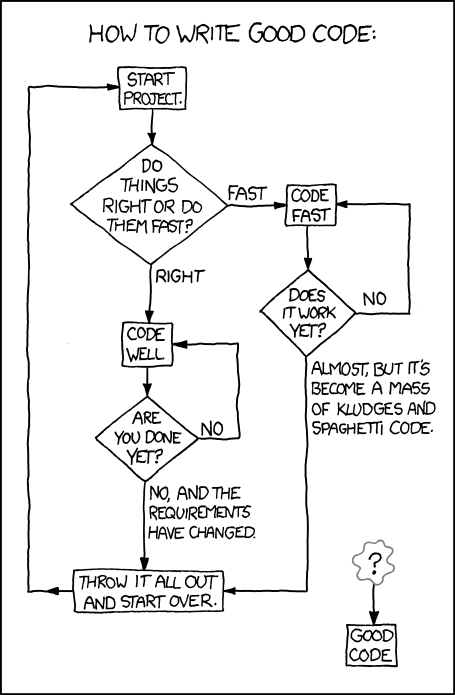
\includegraphics[scale=0.39]{good_code}
        \end{figure}
    \end{columns}
\end{frame}


\begin{frame}
	\frametitle{Quiz}
	\section{Quiz}
	\begin{enumerate}
		\item Write short description of the following: \ (Marks:2 for each part)
		\begin{itemize}
			\item Algorithm
			\item Machine Language
			\item Assembler
			\item Advantages of Debugging?
		\end{itemize}
		\item Advantages of C++ in detail \ (Marks:5)
		\item Applications of Programming \ (Marks:2)
	\end{enumerate}
\end{frame}



\begin{frame}
    \frametitle{Basics of a Typical C++ Environment}
    \section{Basics of a Typical C++ Environment} % (fold)
    \label{sec:environment_basics}
    \begin{columns}
        \column{0.5\textwidth}
        Phases of C++ Programs
        \begin{itemize}
            \item Edit
            \item Preprocess
            \item Compile
            \item Link
            \item Load
            \item Execute
        \end{itemize}
        \column{0.5\textwidth}
            \begin{figure}
                \centering
                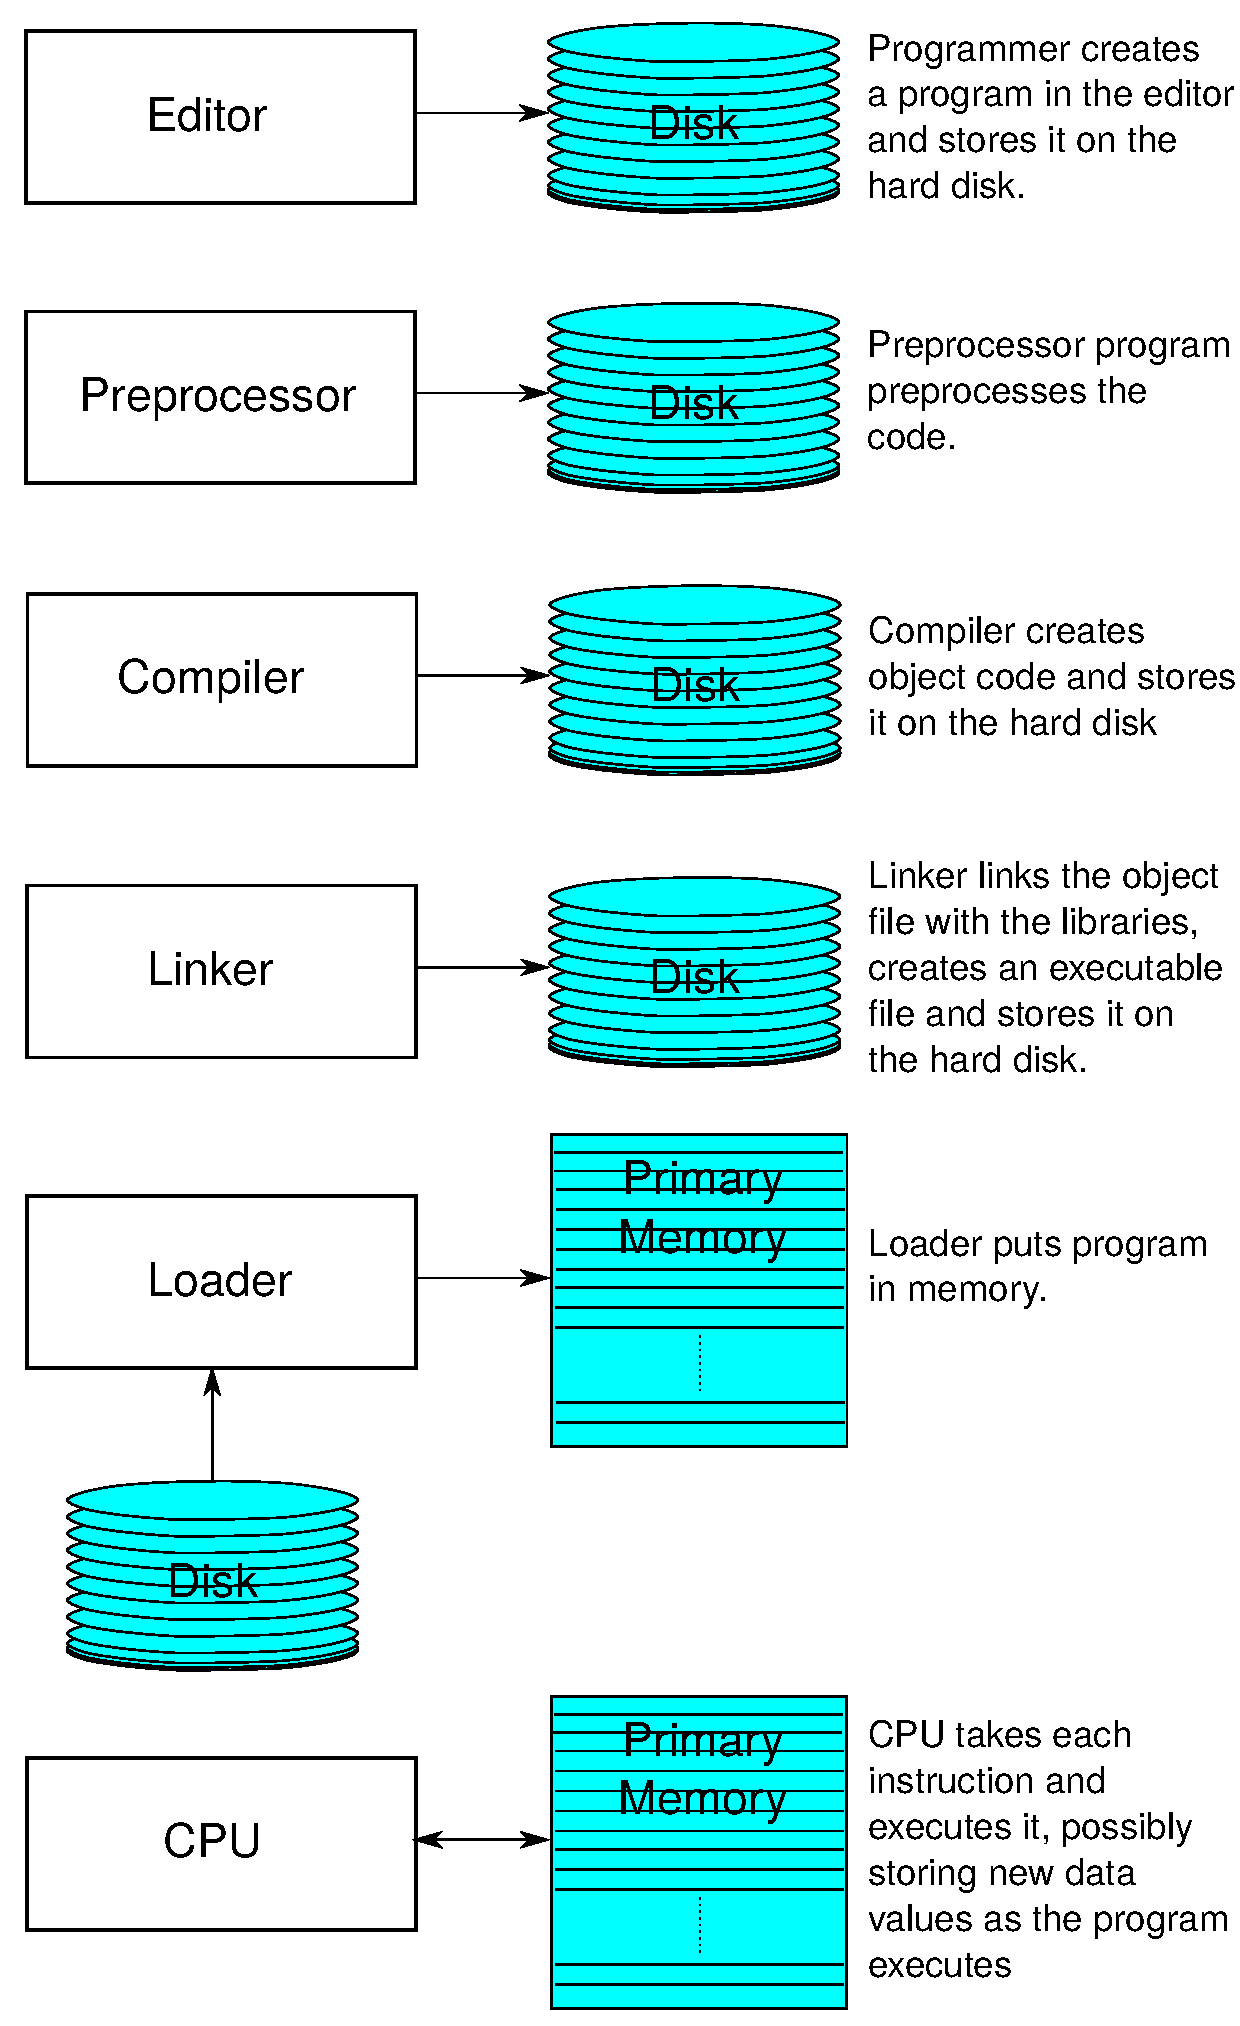
\includegraphics[scale=0.2]{6phases.pdf}
            \end{figure}
    \end{columns}
\end{frame}

\begin{frame}[fragile]
    \frametitle{First Program in C++}
    \section{First Program in C++} % (fold)
    \label{sec:first_program}
    \begin{columns}
        \column{0.57\textwidth}
        \lstset{style=mystyle}
        \begin{lstlisting}
// my first program in C++
#include <iostream>
using namespace std;
int main()
{
    cout << "My First Program!" << endl;
    return 0;
}\end{lstlisting}
        \column{0.42\textwidth}
           \textbf{Line-by-line Explanation}
           \begin{enumerate}
               \item Single line comment. In C++, there are two types of comments.
               \begin{itemize}
                   \item Single line -- //...
                   \item Multi line -- /*...*/
               \end{itemize}
               \item Preprocessor directive to include input/output stream header file.
               \item A namespace where features of the C++ standard library such as \texttt{cout} or \texttt{endl} are declared.
               
           \end{enumerate}
    \end{columns}
\end{frame}

\begin{frame}[fragile]
    \frametitle{First Program in C++}
    \begin{columns}
        \column{0.57\textwidth}
        \lstset{style=mystyle}
        \begin{lstlisting}
// my first program in C++
#include <iostream>
using namespace std;
int main()
{
    cout << "My First Program!" << endl;
    return 0;
}\end{lstlisting}
        \column{0.42\textwidth}
           \textbf{Line-by-line Explanation}
           \begin{enumerate}
           \setcounter{enumi}{3}
           \item Function \texttt{main} appears at least once in every C++ program.
           \item Left brace begins function body.
           \item \texttt{cout} belongs to namespace std and is used for console output, \texttt{<<} is known as a stream insertion operator. \texttt{endl} also belongs to namespace std and is used to insert a newline character.
            \item \texttt{return} statement is used to terminate the execution of a function.
            \end{enumerate}
    \end{columns}
\end{frame}

\begin{frame}
    \frametitle{Arithmetic Operators}
    \section{Arithmetic Operators} % (fold)
    \label{sec:arithmetic}
    \begin{figure}
        \centering
        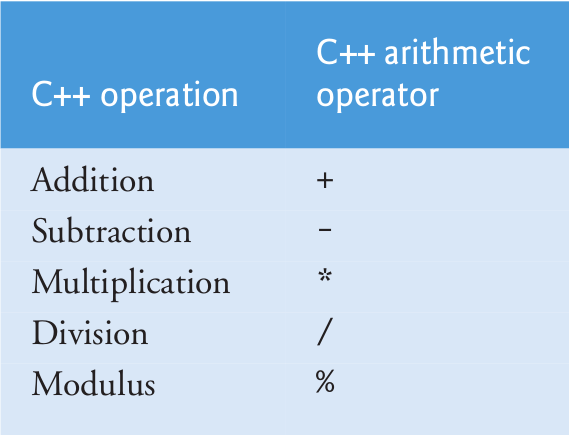
\includegraphics[scale=0.4]{arithematic}
    \end{figure}
\end{frame}

\begin{frame}
    \frametitle{Fundamental C++ Data Types}
    \section{Fundamental C++ Data Types} % (fold)
    \label{sec:fundamental_data_types}
    The C++ language offers several fundamental data types. These include
    \begin{itemize}
        \item \texttt{int} (-2,147,483,648 \textit{to} 2,147,483,647) takes up \textbf{4 bytes}
        \item \texttt{short} (-32,768 \textit{to} 32,767) takes up \textbf{2 bytes}
        \item \texttt{float} ($3.4\times10^{-38}$ \textit{to} $3.4\times10^{38}$) takes up \textbf{4 bytes}
        \item \texttt{double} ($1.7\times10^{-308}$ \textit{to} $1.7\times10^{308}$) takes up \textbf{8 bytes}
       
        \item \texttt{char} (-128 \textit{to} 127) takes up \textbf{1 byte}
    \end{itemize}
\end{frame}

\begin{frame}
    \frametitle{Fundamental C++ Data Types}
    \begin{itemize}
        \item The strong data type system of C++ helps make sure that the data variables are used consistently and correctly.
        \item Type checking makes it easy for the compiler to spot errors during compilation and thus prevent such issues during execution of the program.
        \item Before a variable is used in C++, it must be declared and defined as follows, \\
        \texttt{int myage;}
        \item This line declares and defines a variable named \texttt{myage} as an integer.
    \end{itemize}
\end{frame}

\begin{frame}
    \frametitle{Fundamental C++ Data Types}
    \begin{itemize}
        \item A declaration introduces the name \texttt{myage} to the compiler and attaches a specific meaning to it.
        \item A definition like this also instructs the compiler to allocate some memory for the variable.
    \end{itemize}
\end{frame}

\begin{frame}
    \frametitle{Fundamental C++ Data Types}
    When the compiler reads \texttt{myage} definition,
    \begin{itemize}
        \item It sets aside enough memory storage for an integer and uses the name \texttt{myage} to refer to it.
        \item It reserves the name \texttt{myage} so that it cannot be used by any other variable.
        \item It ensures that whenever this variable is used, it is used in a way that is consistent with the way an integer should be used.
    \end{itemize}
\end{frame}

\begin{frame}
    \frametitle{Keywords in C++}
    \section{Keywords in C++} % (fold)
    \label{sec:keywords}
    \begin{itemize}
        \item Predefined reserved identifiers which have a special significance within the language.
        \item They are case-sensitive and cannot be used as identifiers in your program.
        \item They will be highlighted with a specific color by Visual Studio's editor as you write your code.
        \item If the keywords you type in do not appear highlighted, then they have been entered incorrectly.
    \end{itemize}
\end{frame}

\begin{frame}
    \frametitle{Keywords in C++}
    Here's a list of all the reserved keywords in standard C++.
    \begin{figure}
        \centering
        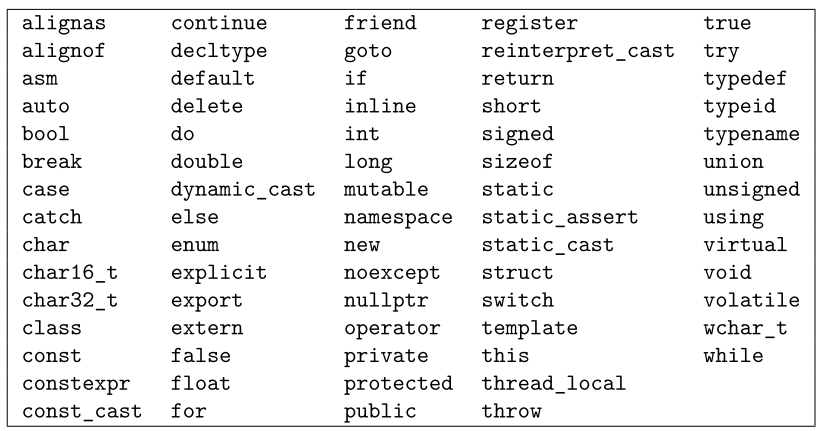
\includegraphics[scale=0.55]{keywords}
    \end{figure}
\end{frame}

\begin{frame}
    \frametitle{Stream I/O}
    \section{Stream I/O} % (fold)
    \label{sec:stream}
    \begin{itemize}
        \item C++ input/output revolves around the notion of a data stream, where we can insert data into an output stream or extract data from an input stream.
        \item The standard output stream to the screen is referred to as \texttt{cout}.
        \item The standard input stream from the keyboard is referred to as \texttt{cin}.
    \end{itemize}
\end{frame}

\begin{frame}
    \frametitle{Assignment Statements}
    \section{Assignment Statements} % (fold)
    \label{sec:assignment}
    \begin{itemize}
        \item The statement which assigns some value to a variable is called an assignment statement.
        \item The $=$ operator is used to assign a value to a variable.
        \item In an assignment statement such as \texttt{myage = 25;}, the variable \texttt{myage} has been assigned a value of \texttt{25}.
    \end{itemize}
\end{frame}

\begin{frame}
\frametitle{What is Flowchart?}
\section{What is Flowchart?}
Graphical representation of Code.
\begin{figure}
        \centering
        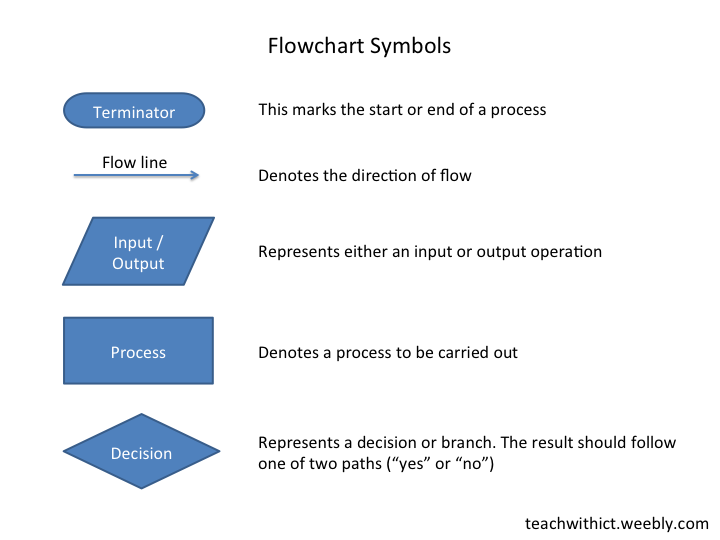
\includegraphics[scale=0.38]{flowchart}
    \end{figure}
\end{frame}


\begin{frame}[fragile]
    \frametitle{Example 1}
    \section{Solved Examples} % (fold)
    \label{sec:solved}
    \begin{columns}
    \column{0.62\textwidth}
    \textbf{Algorithm}
    \begin{enumerate}
        \item Start
        \item Declare variables \texttt{a}, \texttt{b} and \texttt{sum}
        \item Initialize \texttt{a} and \texttt{b} to appropriate values
        \item Add \texttt{a} and \texttt{b} and assign the result to \texttt{sum}
        \item Display \texttt{sum}
        \item Stop
    \end{enumerate}
    \column{0.30\textwidth}
    \textbf{Flowchart}
    \begin{figure}
        \centering
        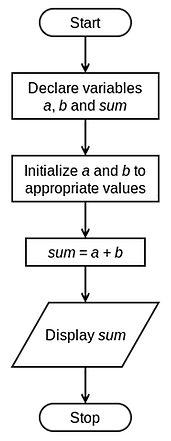
\includegraphics[scale=0.55]{p1flow}
    \end{figure}
    \end{columns}
\end{frame}

\begin{frame}[fragile]
    \frametitle{Example 1}
    \begin{columns}
    \column{0.57\textwidth}
    \textbf{Code}
    \lstset{style=mystyle}
    \begin{lstlisting}
// this program displays the sum of two numbers
#include <iostream>
using namespace std;
int main()
{
    int a, b, sum;
    a = 20;
    b = 30;

    sum = a + b;

    cout << sum << endl;
    return 0;
}\end{lstlisting}
    \column{0.40\textwidth}
    \textbf{Flowchart}
    \begin{figure}
        \centering
        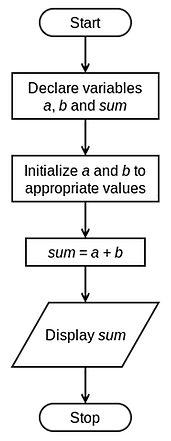
\includegraphics[scale=0.55]{p1flow}
    \end{figure}
    \end{columns}
\end{frame}

\begin{frame}[fragile]
    \frametitle{Example 2}
    \begin{columns}
    \column{0.62\textwidth}
    \textbf{Algorithm}
    \begin{enumerate}
        \item Start
        \item Declare variables \texttt{a}, \texttt{b} and \texttt{sum}
        \item Read values of \texttt{a} and \texttt{b}
        \item Add \texttt{a} and \texttt{b} and assign the result to \texttt{sum}
        \item Display \texttt{sum}
        \item Stop
    \end{enumerate}
    \column{0.30\textwidth}
    \textbf{Flowchart}
    \begin{figure}
        \centering
        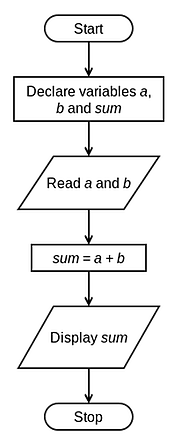
\includegraphics[scale=0.55]{p2flow}
    \end{figure}
    \end{columns}
\end{frame}

\begin{frame}[fragile]
    \frametitle{Example 2}
    \begin{columns}
    \column{0.7\textwidth}
    \textbf{Code}
    \lstset{style=mystyle}
    \begin{lstlisting}
// this program displays the sum of two numbers entered by the user
#include <iostream>
using namespace std;
int main()
{
    int a, b, sum;
    cout << "Enter first number: ";
    cin >> a;
    cout << "Enter second number: ";
    cin >> b;

    sum = a + b;

    cout << "The sum of two numbers is: ";
    cout << sum << endl;

    return 0;
}\end{lstlisting}
    \column{0.26\textwidth}
    \textbf{Flowchart}
    \begin{figure}
        \centering
        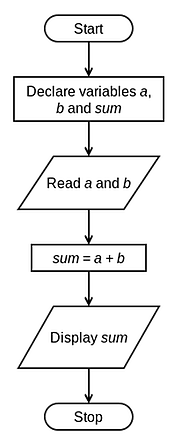
\includegraphics[scale=0.55]{p2flow}
    \end{figure}
    \end{columns}
\end{frame}
\end{document}